\chapter{Desenvolvimento do \frame}\label{chap:software}

O levantamento dos requisitos de um sistema é o elemento que fornece elementos que deve nortear uma série de decisões a serem tomadas no seu desenvolvimento. Primeiramente, apresenta-se aqui o fluxo de trabalho tradicional para análise de fadiga.

\section{Fluxo de avaliação de vida à fadiga sem o \frame}\label{sec:workflow}


Baseado nos estudos e oficinas realizados para o desenvolvimento deste trabalho. Pôde-se estabelecer que a análise de vida à fadiga em dutos em vão-livre compreende o fluxograma apresentado na \autoref{fig:fluxograma}. % chktex 19

\begin{figure}[!ht]
    \centering
    \caption{Fluxo de avaliação de vida à fadiga em dutos em vão-livre.}\label{fig:fluxograma}
    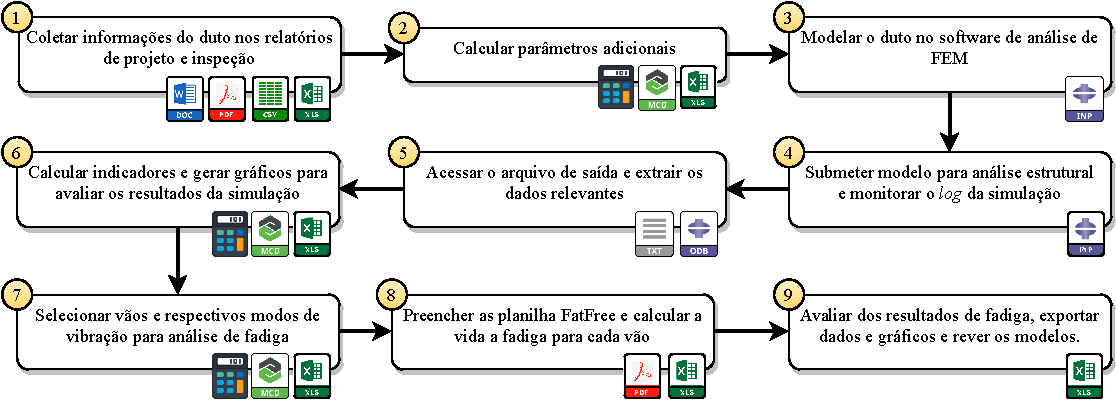
\includegraphics[width=\textwidth]{imagens/fluxograma.pdf}
    \fonte{Autor (2020)}
\end{figure}

A seguir, uma breve descrição de cada item:

\begin{enumerate}[label= (\arabic*)]
    \item Nesta etapa, o profissional reúne as informações básicas para construção dos modelos e outros dados usados em cálculos posteriores. Citadamente, temos aqui: as cotas do perfil do duto e batimetria obtidas na inspeção, geometria e propriedades dos materiais das camadas que compõem sessão do duto, parâmetros do solo, coeficientes de segurança e outras constantes físicas, posição e tipos de suportes ao longo do duto. Essa tarefa envole analisar uma série de documentos (\texttt{.doc}, \texttt{.pdf}, etc) em busca desses valores, dispostos de forma não estruturada. Quando estruturados, em forma de arquivos CSV ou planilhas, por exemplo, é necessário ainda manipular esses dados de modo a extrair somente a informação necessária e/ou convertê-las no formato apropriado. Um exemplo disso são os dados de batimetria, que precisam convertidos nas coordenadas dos nós de uma malha de elementos finitos no formato de um arquivo \texttt{.inp}.---no caso do ABAQUS. De posse desses dados, pode-se então, iniciar a fase de pré-processamento.
    \item Uma vez que nem todos os dados a serem utilizados estão de acordo com as especificações dos softwares a serem empregados nas análises numéricas, ainda é necessários manipular alguns desses valores, seja calculando constantes ou convertendo unidades. Para isso, geralmente utiliza-se softwares de planilhas e/ou folhas de cálculos (Microsoft Excel, MathCad, Maple, etc.). Esta etapa inicia o pré-processamento dos dados.
    \item Com todos os dados em mãos, é necessário transformá-los em um modelo no software de elementos finitos, via interação com mouse e teclado (GUI), ou criando arquivos de entrada. Embora a reutilização de arquivos de entrada previamente criados facilite essa tarefa, nem todos os trechos desses arquivos são suficientes ou podem ser reaproveitados. Estas limitações são frequentes em trechos do arquivo que precisam ser repetidos a depender da quantidade de certas entidades no modelo---suportes, por exemplo. Ao fim desta etapa, encerra-se o pré-processamento dos dados.
    \item Por mais simples que seja submeter o modelo para análise na maioria dos softwares de análise de elementos (alguns cliques via GUI, ou um comando via CLI\footnote{\textit{Command Line Interface}: interface de linha de comando}), as análises costumam levar horas e envolver execuções sucessivas a fim de realizar intervenções no modelo que não podem ser modeladas previamente. Dessa forma, torna-se necessário o monitoramento do progresso da simulação. Esta etapa compreende a primeira parte do processamento propriamente dito.
    \item Uma vez concluída a simulação Análise de Elementos Finitos (FEA, em inglês), é necessário analisar os resultados antes do pós-processamento. Por vezes, é preciso extrair os resultados que estão armazenados em arquivos proprietários (como \texttt{.odb}, no caso do ABAQUS), utilizando as funcionalidades das ferramentas dos próprios pacotes de software de elementos finitos para isso. Esta tarefa, geralmente feita via GUI, costuma ser repetitiva e pode levar de alguns minutos ou horas. Esta etapa inicia parte do pós-processamento da FEA\@.
    \item De posse dos resultados em formatos acessíveis a outros software (MS Excel e MathCad, por exemplo), é necessário calcular (e muitas vezes visualizar em gráficos) alguns indicadores a fim de avaliar a validade dos resultados. Embora poderosos, estes softwares ainda carecem de gráficos mais interativos, como possibilidades de ampliar e transladar os gráficos com o mouse. Esta etapa encerra o pós-processamento da FEA\@.
    \item Na metodologia presente na \dnvf105---que será abordada adiante no \autoref{sec:multimode}---o cálculo de fadiga é baseada em modelos de resposta, portanto, é necessário calcular a resposta de cada modo para as várias condições de carregamento ambiental, o que a torna impraticável sem automação. Para solucionar este problema, foi criada a \fatfree, uma planilha de cálculo comercial que realiza estas operações. No entanto, dentre as dezenas de modos obtidos por solução modal na FEA costumam aparecer modos espúrios. Dessa forma, antes de realizar a análise na \fatfree, é necessário escolher dentre os modos de vibração obtidos na simulação numérica aqueles que mais contribuem para fadiga. Esta tarefa pode ser feita via inspeção visual, observando a forma dos modos, mas é uma prática pouco precisa e subjetiva.
    \item Uma vez selecionados os modos a serem usados para cálculo de fadiga, é necessário o preenchimento da planilha com os dados de deflexão normalizada de cada modos, o que consiste em algumas centenas de valores. Além disso, é necessário preencher muitas outras informações referentes geometria e propriedades dos materiais da sessão do duto, parâmetros do solo, coeficientes de segurança e condições de carregamento em várias páginas diferentes. Com todos os dados preenchidos e opções selecionadas nos controles da planilha, pode-se apertar o botão que calcula os resultados de fadiga.
    \item Finalmente, os dados de fadiga pode ser analisados e exportados para outras ferramentas a fim de gerar relatórios.
\end{enumerate}


\section{Fluxo de avaliação de vida à fadiga com uso do \frame}


O \frame\ proposto tem como requisito atender o fluxo apresentado na \autoref{sec:workflow}, automatizando certas etapas da análise de vida à fadiga. Os itens coloridos são cobertos pela implementação \frame, e os itens  branco são realizados em aplicações externas.


\begin{figure}[!ht]
    \centering
    \caption{Fluxo de operação proposto para o \frame.}\label{fig:workflow}
    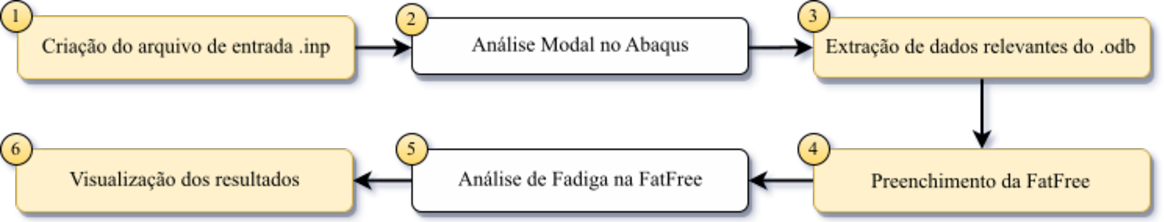
\includegraphics[width=\textwidth]{imagens/fluxograma_automatizado}
\end{figure}

De forma mais detalhada, a ferramente deve:

\begin{enumerate}[label= (\arabic*)]
    \item A partir de um arquivo de entrada com informações do modelo, criar arquivos de entrada para o ABAQUS (.inp) que reproduza todo o processo de simulação do comportamento do duto apresentado (\autoref{sec:assentamento}).
    \item Submeter o arquivo gerado para análise no ABAQUS. No caso de haver a colocação de suportes, a simulação é executada em duas partes: a primeira com os passos de carga anteriores a passo da colocação dos suportes, e a segunda com o passo da colação dos mesmos e os passos de carga seguintes.
    \item Processar os arquivos de saída do ABAQUS (.odb) extraindo as informações relevantes como a configuração deformada, modos de vibração, etc., gerando arquivos em outros formatos de fácil leitura para pós-processamento, tanto por este \frame, quanto por outros softwares.
    \item Pós-processar as informações gerando gráficos e relatórios relevantes para as tomadas de decisão do usuário quanto ao projeto. Esse é o requisito mais crítico, uma vez que é fundamental o entendimento sobre a análise de duto em vão-livre. Entre as tarefas que fazem parte deste item está a automação da escolha dos modos de vibração ativos e relevantes e para cada vão de interesse --- a qual deve ser norteada pelos aspectos discutidos na \autoref{sec:multimode} --- e a manipulação da FatFree.
    \item Ativar o processo de cálculo de fadiga no arquivo preenchido no passo anterior.
    \item Capturar os resultados no arquivo \texttt{.xls} da \fatfree, que agora contém os resultados do cálculo de vida à fadiga, e apresentá-los na forma de gráficos e relatórios.
\end{enumerate}


\section{Implementação computacional}


\subsection{Linguagem de programação}

Python\footnote{https://www.python.org} foi a linguagem de programação adotada. Além de ser uma linguagem interpretada de alto nível Orientada a Objeto --- que permite um alto índice de reaproveitamento de código --- e da sintaxe simples. \citeonline{Rao2018} apresenta algumas das principais vantagens que destaca a linguagem para este tipo de aplicação:

\begin{itemize}
    \item Disponibilidade de bibliotecas para aplicações científicas contemplando manipulação de matrizes (Numpy), funções matemáticas (SciPy), manipulação de dados em forma tabular (Pandas), criação de gráficos interativos (Matplotlib e Bokeh).

    \item Suporte para automação de tarefas. Os recursos de \textit{script} internos do Python e vários pacotes têm um forte suporte à automação de tarefas. A automação de tarefas repetitivas e a realização do registro de dados são fáceis e requerem pouco esforço. O ABAQUS, por exemplo, permite modelagem e acesso a informações em arquivos de saída via Python. A biblioteca xlwings permite manipulação de planilhas Excel, a exemplo da FatFree.

    \item Pacotes Python como Django e Flask tornam possível desenvolver e usar o Python como uma API\footnote{Na programação de computadores, uma Interface de Programação de Aplicativos (\textit{Application Programming Interface}---API) é um conjunto de definições de sub-rotinas e ferramentas para a criação de software. Em termos gerais, é um conjunto de métodos de comunicação claramente definidos entre vários componentes.} com um \textit{front-end} da web. Essa funcionalidade é particularmente útil para reaproveitamento do \frame\  em outras aplicações.
\end{itemize}


\subsection{Pacotes e classes}


Para implementação do fluxo de trabalho proposto para o \frame, fez-se a implementação de módulos para lidar com cada contexto específico. Em python, módulos podem ser quaisquer arquivos com extensão \texttt{.py}. Estes módulos podem ser agrupados em pacotes, que são pastas que, além dos módulos, contém um arquivo \texttt{\_\_init\_\_.py}. No \frame\ têm-se alguns pacotes que agrupam módulos em torno do contexto de um problema que o \textit{software} resolve. % chktex 21


\subsubsection{Pacote \texttt{analysis}}


É o pacote principal responsável orquestrar o fluxo de trabalho do \frame\ desde o processamento dos dados de entrada, geração dos arquivos para o ABAQUS e os pós-processamentos. As funções de pré-processamento de dados estão aqui. Este pacote tem dois módulos (\texttt{models.py} e \texttt{inp.py}) que contém duas classes principais, respectivamente:

\begin{itemize}
    \item \texttt{Model}: classe que contém as informações do modelo do problema.
    A classe armazena todas as informações para construção dos arquivos \texttt{.inp}, isto é, dados de batimetria, material, geometria do duto, coeficientes de segurança, entre outros.
    A principal forma de criação da instâncias dessa classe é pelo método estático \texttt{load\_json}, que recebe um arquivo principal de entrada (em formato JSON, ver \autoref{apendice:json}), e realiza o pré-processamento dos dados contidos nele.

    \item \texttt{Inp}: lida com a escrita modularizada de arquivos de entrada  para o ABAQUS. A proposta é que se tenha um arquivo \texttt{.inp} principal que terá conterá informações para a localização de outros arquivos acessórios que, por sua vez, terão as informações específicas de cada aspecto da modelagem: batimetria, passos de carga, etc. Isso facilita o reaproveitamento dos arquivos acessórios, sem precisa de alterações no arquivo principal.
\end{itemize}

A \autoref{fig:analysis-uml} exibe um diagrama UML\footnote{Sigla para \textit{Unified Modeling Language}: Linguagem Unificada de Modelagem é uma linguagem padrão para modelagem orientada a objetos~\cite{infoescolauml}} com uma visão geral do pacote \texttt{analysis}.

\begin{figure}[!ht]
    \centering
    \caption{Digrama UML do pacote \texttt{analysis}.}\label{fig:analysis-uml}
    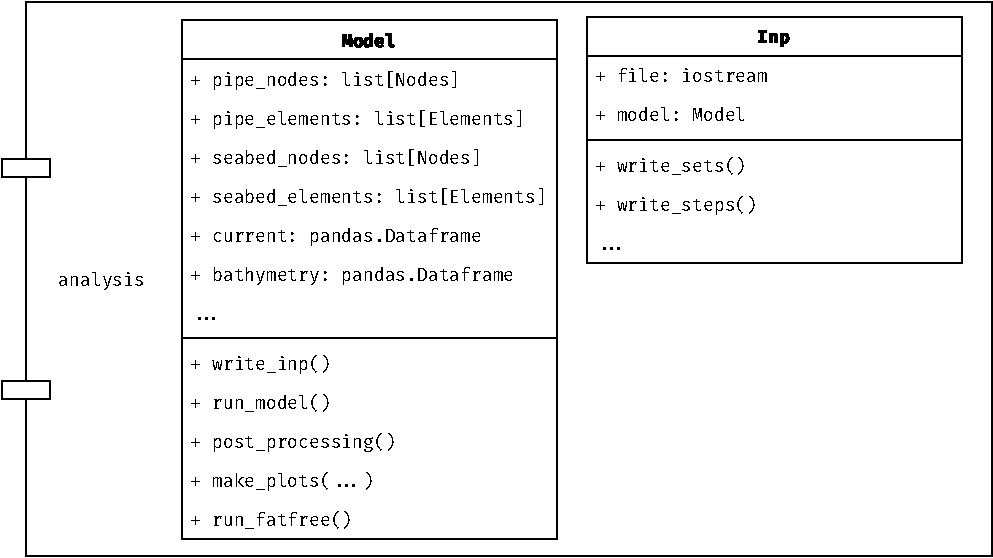
\includegraphics[width=0.8\textwidth]{imagens/analysis-uml}
    \fonte{Autor (2020)}
\end{figure}


\subsubsection{Pacote \texttt{odb\_handler}}


Neste pacote está o módulo responsável por lidar com os arquivos de saída do ABAQUS (odb) no sentido de acessar e guardar os dados relevantes em arquivos com formatos de fácil manipulação por outros softwares (CSV e JSON, por exemplo, que possui módulos para leitura e escrita nativos em Python).

% A \autoref{fig:odb-handler-uml} exibe um diagrama UML com uma visão geral do pacote \texttt{odb\_handler}.

\begin{figure}[!ht]
    \centering
    \caption{Digrama UML do pacote \texttt{odb\_handler}.}\label{fig:odb-handler-uml}
    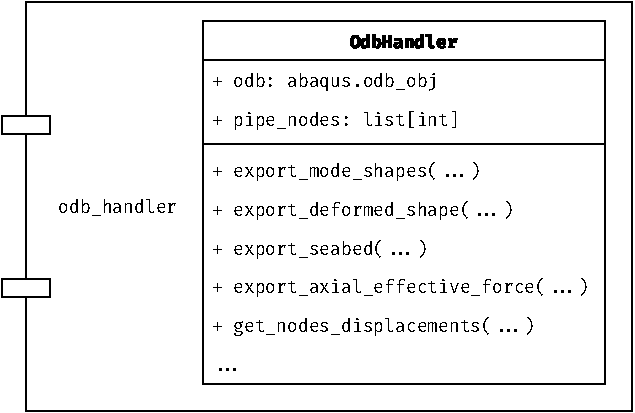
\includegraphics[width=0.5\textwidth]{imagens/odb-handler-uml}
    \fonte{Autor (2020)}
\end{figure}


\subsubsection{Pacote \texttt{mode\_selector}}


Neste pacote estão implementados os métodos responsáveis pela estratégia de seleção automática de modos de vibração (que depende da definição dos vãos), bem como e manipulação dos dados associados vãos e seus respectivos modos. As abstrações dos conceitos de vão e modo de vibração estão implementadas nas seguintes classes:

\begin{itemize}
    \item \texttt{Span}: classe que representa um vão do duto. Uma vez que análise de fadiga é feita por vão, é nesta que são implementados os métodos responsáveis pela seleção dos modos de vibração, que são ligados à classe por um dos seus atributos.

    \item \texttt{ModeShape}: classe que representa um modo de vibração (\textit{mode shape}). A principal forma de criação de objetos dessa classe é por meio da função \texttt{load\_json} do módulo \texttt{mode\_shapes.py}, que carrega os dados do arquivo gerado com utilização do \texttt{odb\_handler}, e retorna uma lista de objetos desta classe.
\end{itemize}

A \autoref{fig:mode-selector-uml} exibe um diagrama UML com uma visão geral do pacote \texttt{mode\_selector}.

\begin{figure}[!ht]
    \centering
    \caption{Digrama UML do pacote \texttt{mode\_selector}.}\label{fig:mode-selector-uml}
    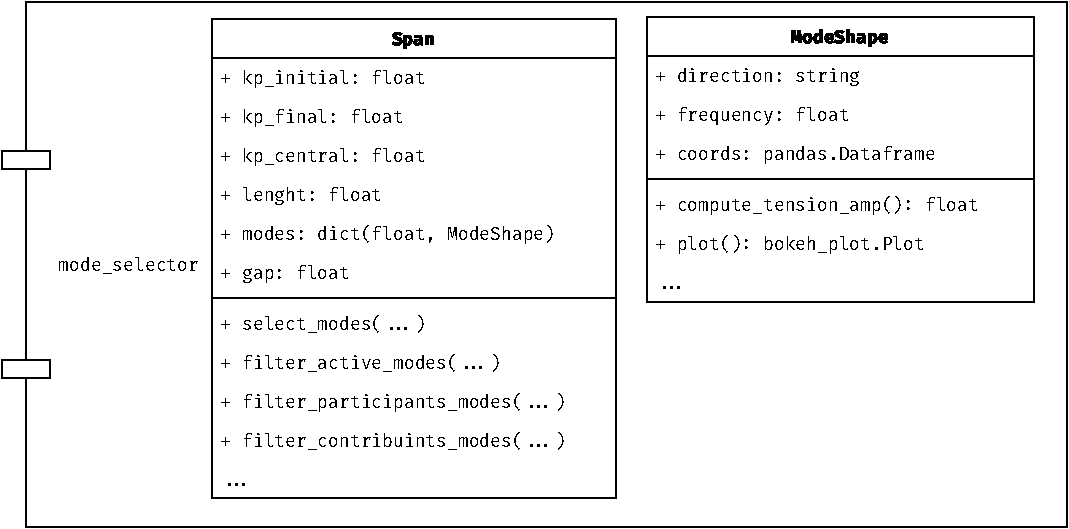
\includegraphics[width=0.8\textwidth]{imagens/mode-selector-uml}
    \fonte{Autor (2020)}
\end{figure}


\subsubsection{Pacote \texttt{dnv}}

Neste pacote são agrupadas módulos referentes à \dnvf105, como cálculos dos modelos de resposta da \dnvf105, subsidiam o algorítmo de seleção de modos de vibração, e entrada de saída de dados da planilha FatFree. As principais classes contidas nesses pacotes são:

\begin{itemize}
    \item \texttt{ResponseModel}: implementa formulação dos modelos de resposta apresentados na \autoref{sec:viv}.

    \item \texttt{FatFree}: responsável fazer a entrada dos dados na planilha e invocar a execução dos cálculos. Essa classe faz uso da biblioteca \texttt{Xlwings}, que consegue se comunicar com o Microsoft Excel e manipular os componentes (caixas de seleção, botões, etc) que formam a interface da FatFree.

    \item \texttt{FatFreeResults}: Esta classe permite o acesso facilita o acesso programático aos dados contidos em um determinado aqui da FatFree.
\end{itemize}

A \autoref{fig:dnv-uml} exibe um diagrama UML com uma visão geral do pacote \texttt{dnv}.

\begin{figure}[!ht]
    \centering
    \caption{Digrama UML do pacote \texttt{dnv}.}\label{fig:dnv-uml}
    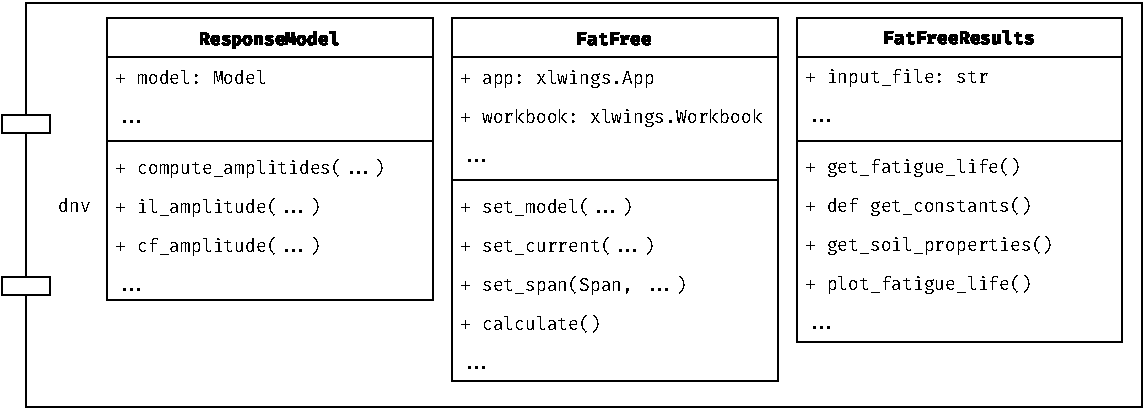
\includegraphics[width=\textwidth]{imagens/dnv-uml}
    \fonte{Autor (2020)}
\end{figure}


\subsubsection{Pacote \texttt{plots}}


Pacote responsável pro agregar as funções de geração de gráficos dos resultados. Disponibilizar essas funções dentro do \frame permite que os gráficos com os resultados das análises sejam gerados automaticamente, o visual e forma de apresentação sejam padronizados. As principais classes neste pacote são:

\begin{itemize}

    \item \texttt{Plot}: é construída em cima da classe \texttt{Figure} da biblioteca \texttt{Bokeh}\footnote{www.bokeh.org}, que permite a criação de gráficos interativos em HMTL. Os gráficos gerados por essa biblioteca possuem controles permitem, por exemplo, que o usuário dê zoom ou translate os dados exibidos, ative/desative os ítem mostrado por meio de clique nos respectivos itens nas legendas, sabe o gráfico em formato de imagem estática (\texttt{png}). A \autoref{fig:exemplo-bokeh} exibe um exemplo desses gráficos destacando os elementos interativos em vermelho.

    \begin{figure}[!ht]
        \centering
        \caption{Exemplo de gráfico customizado criado com a biblioteca Bokeh.}\label{fig:exemplo-bokeh}
        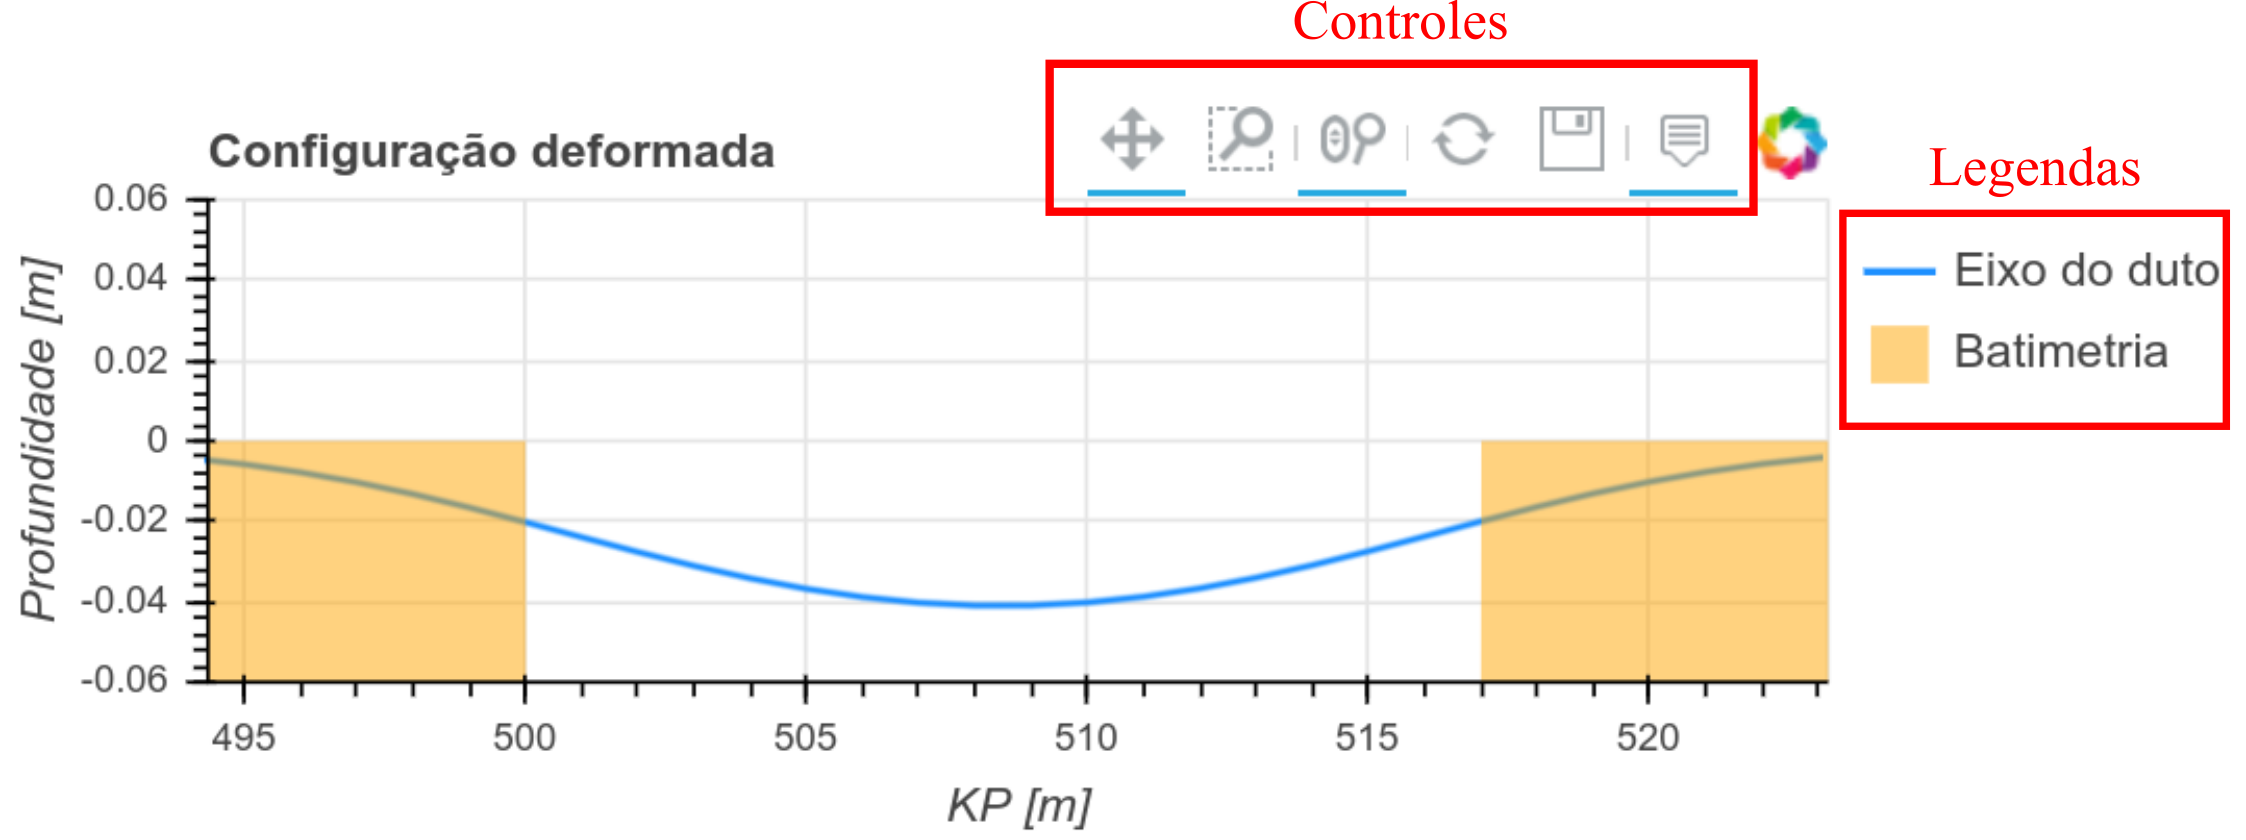
\includegraphics[width=0.8\textwidth]{imagens/exemplo-bokeh}
        \fonte{Autor (2020)}
    \end{figure}

    O trabalho da classe \texttt{Plot} é simplificar a criação dos gráficos devido a implementação de métodos que facilitam desde alterar os componentes mais comuns das figuras, como títulos dos eixos e legendas, até combinar gráficos e formar \textit{dashboards} com gráficos integrados. A combinação de gráficos pode ser feita por meio dos operadores matemáticos:
    \begin{itemize}
        \item \texttt{a + b}: para sobrepor os gráficos \texttt{a} e \texttt{b};
        \item \texttt{a | b}: para posicionar dois gráficos, com \texttt{a} à esquerda de \texttt{b};
        \item \texttt{a / b}: para posicionar dois gráficos, com \texttt{a} acima de \texttt{b};
    \end{itemize}

    \item \texttt{PipeProfileDashboards}: esta classe se utilizada da classe \texttt{Plot} para facilitar a criação de um tipo \textit{dashboard} recorrente no processo de análise: dois gráficos empilhados verticalmente, um com dados que podem ser associados a posição ao longo do duto (como esforço axial, modos de vibração, enterramento, vida à fadiga, etc), e o outro abaixo dele com o perfil do duto. Nesse tipo de arranjo é interessante que os eixos das abcissas estejam atrelados, permitindo ao usuário movimentar os dois eixos em sincronia.
\end{itemize}

A \autoref{fig:plots-uml} exibe um diagrama UML com uma visão geral do pacote \texttt{plots}.

\begin{figure}[!ht]
    \centering
    \caption{Digrama UML do pacote \texttt{plots}.}\label{fig:plots-uml}
    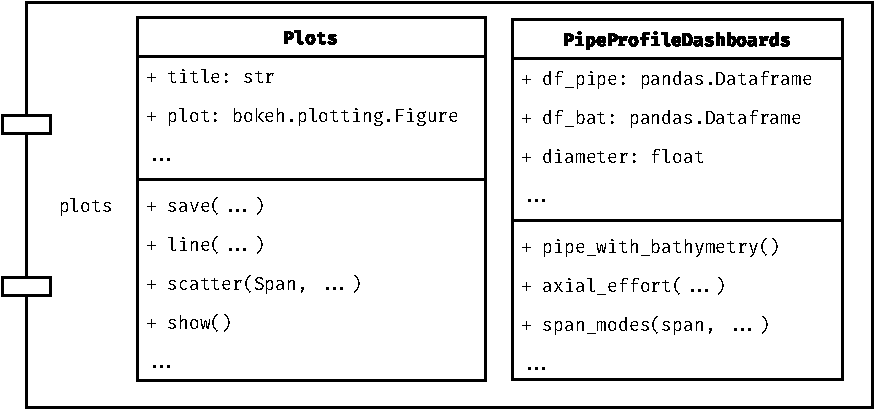
\includegraphics[width=0.7\textwidth]{imagens/plots-uml}
    \fonte{Autor (2020)}
\end{figure}